%% ------------------------------------------------------------------------- %%
\chapter{Abordagem}
\label{cap:abordagem}

Conforme citado no Capítulo~\ref{cap:fundamentacao-teorica}, uma técnica muito utilizada para \textit{code retrieval} é a \textit{joint embedding}. Para utilizar esta técnica, três fatores devem ser levados em consideração:

\begin{itemize}
    \item Representação de cada palavra de uma sentença ou trecho de código-fonte
    \item Representação da sentença e do trecho de código-fonte
    \item Função objetivo do modelo
\end{itemize}

A nossa proposta é criar um modelo que faz uso das redes convolucionais na aprendizagem de representação das questões e trechos de código-fonte. Porém, conforme levantado anteriormente, outros aspectos também devem ser levados em consideração. Como as palavras serão representadas e qual função objetivo utilizaremos para que o modelo induza a aproximação das questões aos trechos de código-fonte que são solução. Então, neste capítulo, apresentaremos a nossa abordagem para cada um destes itens.

\section{Representação de cada palavra de uma sentença ou trecho de código-fonte}
\label{sec:abordagem-representacao-token}

As questões e os trechos de código-fonte são compostos por palavras, pontuações, separadores e caracteres de símbolos e operadores matemáticos. Para as questões, que são descritas em linguagem natural, iremos representá-las como um vetor formado por uma sequência de palavaras, apenas removendo os caracteres de acento e pontuação.

No caso do código-fonte, iremos partir da  mesma hipótese que utilizamos no artigo \cite{marcelo-vem-2019}, apresentado no \acrfull{vem}. Essa hipótese foi levantada por \cite{Allamanis:2018:SML} e diz que software é uma forma de comunicação humana e tem propriedades estatísticas similares a corpora de linguagem natural. A partir disto, iremos aplicar os mesmos procedimentos adotados para as questões aos trechos de código-fonte. Quer dizer, os trechos de código-fonte serão tratados como uma sequência de palavras e terão os acentos e caracteres especiais removidos.

Para cada palavra devemos definir uma representação. Uma boa representação para as palavras são os vetores de representação distribuída. Pois, segundo \cite{Goodfellow-et-al-2016:representation-learning}, as redes neurais generalizam bem quando as palavras são representadas através de vetores de representação distribuída. E conforme os próprios autores, uma boa representação deve auxiliar na aprendizagem de uma tarefa posterior. No nosso caso, as representações devem auxiliar a tarefa de aprender a encontrar uma correlação entre as questões e os trechos de código-fonte mais relevantes.

Portanto, neste trabalho, cada palavra será representada através de um vetor de representação distribuída. Para mapeá-las, utilizaremos, inicialmente, o algoritmo \textit{word2vec}. Ele será utilizado com \textit{skip-gram}, que prediz as palavras do contexto a partir de uma palavra alvo. Segundo \cite{mikolov2013distributed}, \textit{skip-gram} obteve um desempenho melhor em problemas semânticos, e.g., relacionar uma palavra masculina com a equivalente feminina, relacionar o nome de uma capital a um país ou cidade a um estado. No caso do código-fonte, isto é uma característica importante, pois pode ajudar a agrupar os \textit{tokens} de acordo com o tipo. Por exemplo, agrupar a instrução de decisão \textit{while} próxima da instrução \textit{for}. E relacionar a instrução de decisão \textit{if} próxima da \textit{else}.

No nosso caso, o \textit{word2vec} irá mapear cada palavra para um espaço vetorial $\mathbb{R}^{d}$. Seja $\mathbb{Q}$ o conjunto formado pelas palavras das questões e $\mathbb{C}$ o conjunto constituído pelas palavras presentes nos trechos de código-fonte. Para cada palavra ${q} \in \mathbb{Q}$ e palavra ${c} \in \mathbb{C}$ teremos:

\begin{equation}
    f: {q} \rightarrow t_{q}, t_{q} \in \mathbb{R}^{d}
\end{equation}

\begin{equation}
    g: {c} \rightarrow t_{c}, t_{c} \in \mathbb{R}^{d}
\end{equation}
Onde $f$ e $g$ são o \textit{word2vec} com o algoritmo \textit{skip-gram}. $f$ e $g$ irão mapear cada palavra pertencente a um vocabulário a uma matriz distinta $\bm{T_{q}}$ e $\bm{T_{c}}$.
Teremos duas matrizes: $\bm{T}_{q}^{|\mathbb{Q}| X d}$ e outra $\bm{T}_{c}^{|\mathbb{C}| X d}$, onde $|\mathbb{Q}|$ e $|\mathbb{C}|$ são o tamanho do vocabulário das questões e trechos de código-fonte, respectivamente. E $d$ é a dimensão do vetor de representação distribuída.

Com estas duas matrizes $\bm{T}_{q}$ e $\bm{T}_{c}$, que contém as palavras dos vocabulários das questões e dos trechos de código-fonte mapeadas, podemos representar uma sentença através de vetores de representação distribuída. Por exemplo, dado uma questão $\bm{s} = \{ w_{0}, w_{1}, . . ., w_{n - 1}\}$, onde $w_{i}, 0 \leq i < n$ é uma palavra. Podemos representar $\bm{s}$ através de um outro vetor $\bm{x}$, onde para cada palavra presente em $\bm{s}$, elas serão representadas através de um vetor de representação distribuída em $\bm{x}$. Para isto, basta recuperar o vetor $t_{q} \in \bm{T}_{q}$ correspondente a cada palavra presente em nossa questão. Logo, temos $\bm{x} = \{ x(w_{0}), x(w_{1}), . . ., x(w_{n - 1})\}$, tal que $x(w_{i}) \in \bm{T}_{q}$ e $\bm{x}(w_{i}) \in \mathbb{R}^{d}$ é um vetor de representação distribuída. Com o vetor $\bm{x}$, o próximo passo é combinar os seus elementos para obter uma representação da sentença.





\section{Representação da sentença e do trecho de código-fonte}
\label{sec:representacao-sentenca}

Com cada palavra representada por um vetor de representação distribuída, o próximo passo é combiná-las para obter uma representação para a questão e o trecho de código-fonte. Por exemplo, dado uma sentença $\bm{x} = \{ \bm{x}(0), \bm{x}(1), . . ., \bm{x}(n - 1) \}$, onde $\bm{x}(i) \in \mathbb{R}^{d}$ um vetor de representação distribuída da $i^{th}$ palavra da sentença, $d$ é a dimensão do vetor. Iremos combinar os elementos de $\bm{x}$ através das operações presentes em nossa arquitetura CNN. Basicamente são 3 operações:

\begin{itemize}
    \item Operação de convolução
    \item Concatenação
    \item \textit{Maxpool}
\end{itemize}

A operação de convolução utiliza um filtro convolucional $\bm{F}  = [\bm{F}(0),· · ·, \bm{F}(m - 1)]$, tal que $\bm{F} \in \mathbb{R}^{m X d}$. Este filtro é aplicado em uma janela de $m$ palavras para produzir um novo vetor.
Seja $\bm{x}(i, i + j)$ referência a concatenação dos vetores $\bm{x}(i), \bm{x}(i + 1), . . ., \bm{x}(i + j)$. . Ao aplicar $\bm{F}$ na seguinte janela de palavras $\bm{x}(i, i + m - 1)$, um novo vetor $\bm{c}(i)$ é calculado da seguinte maneira:

\begin{equation}\label{eq:calc_convolution_ci}
    \bm{c}(i) = tanh \left[\left(\sum_{j=0}^{m - 1} \bm{x}(i + j)^{T}\bm{F}(j)\right) + b\right]
\end{equation}

onde $b$ é o \textit{bias} e $\bm{F}$ e $b$ são parâmetros do filtro. Para exemplificar esta operação, as figuras~\ref{fig:first-step-convolutional} e \ref{fig:second-step-convolutional} abaixo ilustram um exemplo dos dois primeiros passos da aplicação de um filtro convolucional $\bm{F} \in \mathbb{R}^{m X d}$, onde $m = 2$ e $d = 5$. Este filtro é aplicado a uma sentença formado por 6 palavras, que é representado pelo vetor de representação distribuída $\bm{x} \in \mathbb{R}^{n X d}$, onde $n = 6$ e $d = 5$. Pelas figuras, podemos perceber que o parâmetro $m$ do filtro $\bm{F}$ define como as palavras são combinadas. Neste caso, foram combinadas de duas em duas, um bi-gram.

\begin{figure}[h]
    \centering
    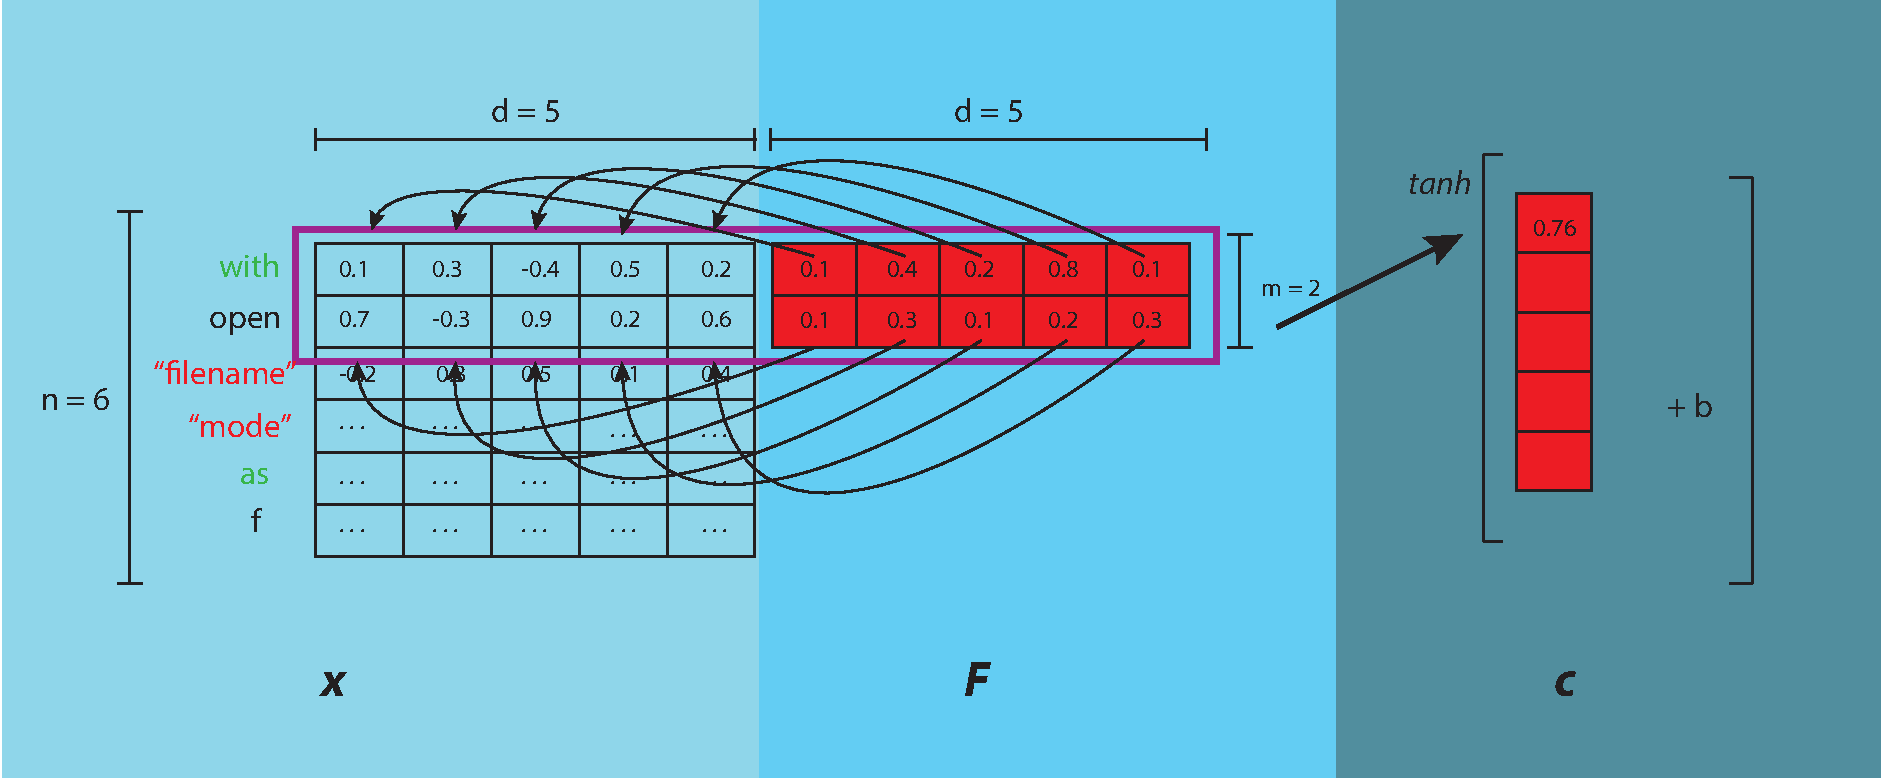
\includegraphics[width=1\textwidth]{figuras/cap-problema/first-step-convolution.pdf}
    \caption{Primeiro passo da operação de convolução. Aplica-se um filtro convolucional $\bm{F} \in \mathbb{R}^{m X d}$, onde $m = 2$ e $d = 5$, em uma sentença $\bm{x} \in \mathbb{R}^{n X d}$, onde $n = 6$ e $d = 5$. Este primeiro passo é equivalente a seguinte operação: $\bm{c}(\bm{0}) = tanh \left[\left(\sum_{j=0}^{m - 1} \bm{x}(\bm{0} + j)^{T}\bm{F}(j)\right) + b\right]$. Figura adapatada a partir do texto de \cite{joshua-kim-cnn-understanding-word-embeddings-2019}.} 
    \label{fig:first-step-convolutional}
\end{figure}

\begin{figure}[h]
    \centering
    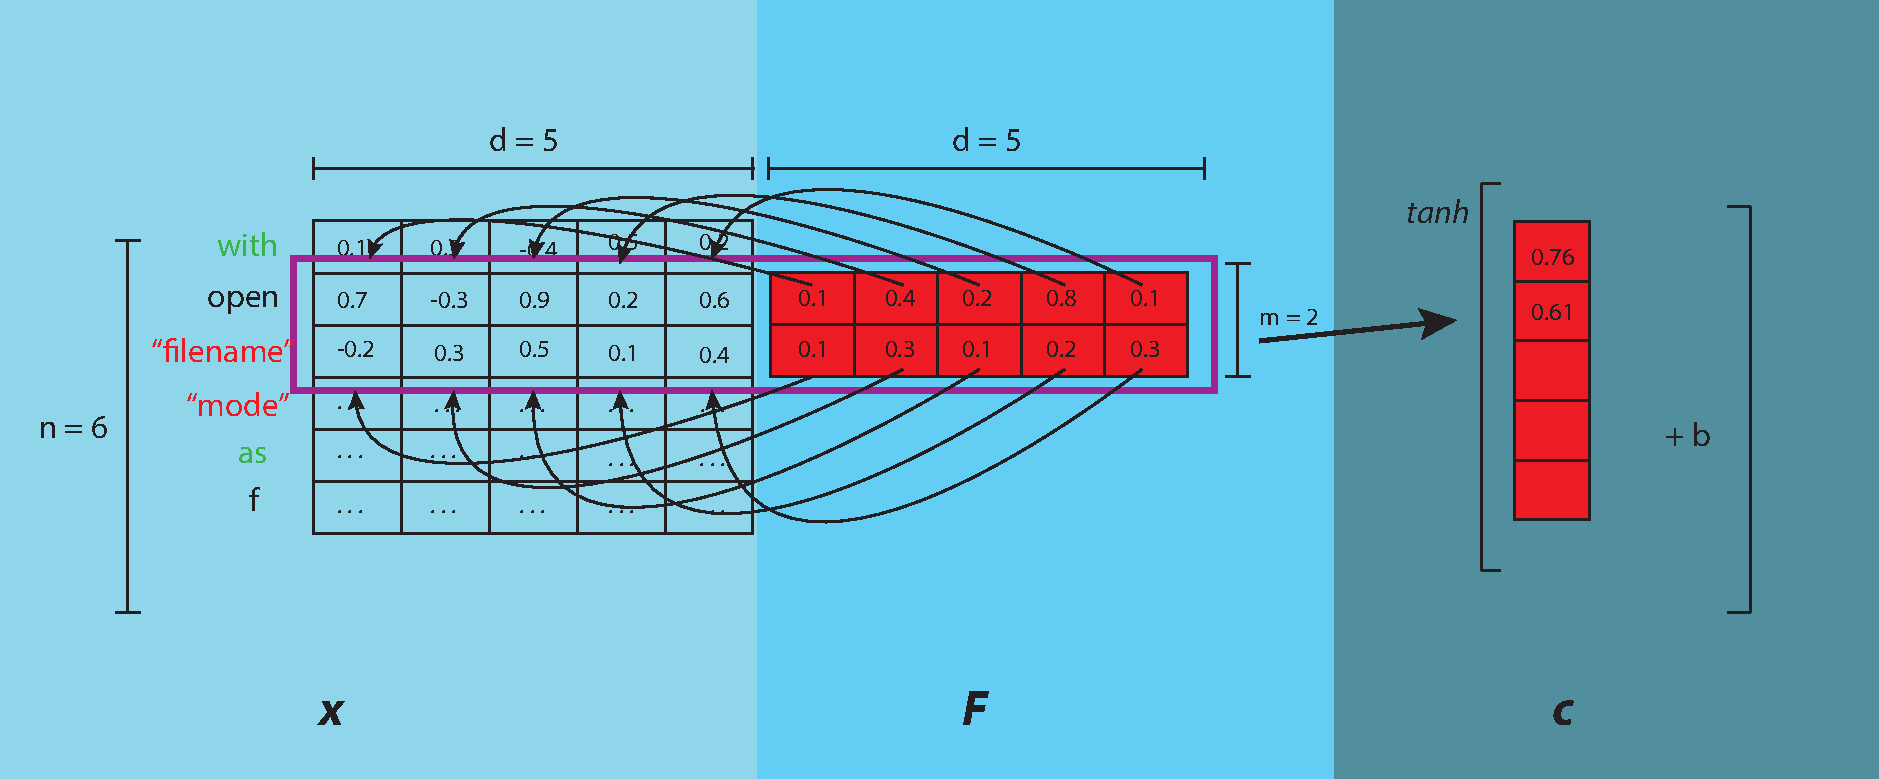
\includegraphics[width=1\textwidth]{figuras/cap-problema/second-step-convolution.pdf}
    \caption{Segundo passo da operação de convolução. Aplica-se o mesmo filtro convolucional $\bm{F} \in \mathbb{R}^{m X d}$, onde $m = 2$ e $d = 5$, em uma sentença $\bm{x} \in \mathbb{R}^{n X d}$, onde $n = 6$ e $d = 5$. Neste segundo passo, deslocamos uma posição no eixo $0$. Este segundo passo é equivalente a: $\bm{c}(\bm{1}) = tanh [(\sum_{j=0}^{m - 1} \bm{x}(\bm{1} + j)^{T}\bm{F}(j)) + b]$. Figura adapatada a partir do texto de \cite{joshua-kim-cnn-understanding-word-embeddings-2019}.}
    \label{fig:second-step-convolutional}
\end{figure}


Durante a operação de convolução, o filtro $\bm{F}$ é aplicado a todas possíveis janelas de palavras utilizando os mesmos pesos para produzir um mapa das características (\textit{feature map}).

\begin{equation}
    \bm{c} = \{ \bm{c}(0), \bm{c}(1), . . ., \bm{c}(n - m) \} 
\end{equation}




Em uma arquitetura CNN, existem centenas de filtros convolucionais $\bm{F}$, também chamados de \textit{kernel}, de diferentes tamanhos $m$ que percorrem toda uma sentença $\bm{x}$. Cada \textit{kernel} extrai características específicas de n-gram. Após a operação de convolução, i.e., o cálculo de $\bm{c}$, realizamos a concatenação dos vetores de saída dos diferentes filtros.
Esta operação de concatenação é realizada apenas entre os filtros que tem diferentes tamanhos de janela, conforme ilustra a Figura~\ref{fig:cnn-architecture-proposal}.
Então para $k$ tamanhos de janelas diferentes, a operação de concatenação irá gerar um vetor $\bm{c}_{\bm{m}}$ através da junção dos $k$ vetores de saída diferentes.

\begin{equation}\label{eq:concatenacao-cnn-cm}
    \bm{c}_{\bm{m}} = \left[\bm{c}_{m_1}, \bm{c}_{m_2}, . . ., \bm{c}_{m_{k}}\right]
\end{equation}

Onde $\bm{c}_{\bm{m}}$ é o resultado da concatenação dos diferentes vetores $\bm{c}$, $\bm{m}$ é um vetor com os diferentes tamanhos de janela, $\bm{m} = \{m_1, m_2, . . ., m_{k}\}$, e $k$ é a quantidade de elementos. Somente ao final que aplicamos a camada \textit{maxpool}. A camada \textit{maxpool} aplica a operação \textit{max}, obtendo o vetor de representação final da sentença $\bm{c'}_{\bm{m}}$. A operação \textit{max} é aplicada no eixo $0$, conforme ilustra a Figura~\ref{fig:cnn-architecture-proposal}. Portanto o vetor final $\bm{c'}_{\bm{m}}$ é obtido da seguinte maneira:

\begin{equation}
    \bm{c'}_{\bm{m}} = max\left(\left[\bm{c}_{m_1}, \bm{c}_{m_2}, . . ., \bm{c}_{m_k}\right], axis = 0\right)
\end{equation}

Onde $axis$ define ao longo de qual eixo a função será aplicada. De forma equivalente, $\bm{c'}_{\bm{m}}$ poderia ser calculado do seguinte modo:

\begin{equation}\label{eq:final_representation_cnn}
    \bm{c'}_{\bm{m}} = \left[max(\bm{c}_{m_1}), max(\bm{c}_{m_2}), . . ., max(\bm{c}_{m_k})\right]
\end{equation}

A operação \textit{max} reduz a dimensionalidade extraindo o maior elemento de cada vetor. Esta redução da dimensionalidade é um fator importante para problemas de classificação, por exemplo. Independente do tamanho da entrada e do filtro, a dimensão da camada de saída vai ser mantida. Além disso, a camada \textit{maxpool} é invariante a pequenas translações. Isto permite extrair características relevantes (e.g. palavras referindo-se a leitura de arquivo: \emph{file} e \emph{open}) de uma sentença independente da sua localização e adiciona-las na representação final \citep{tom-young:trends-deep-learning-nlp}.

Para exemplificar a operação completa, a Figura~\ref{fig:cnn-architecture-proposal} a seguir ilustra um exemplo da aplicação de diferentes filtros convolucionais com diferentes tamanhos de janela $m$ em uma sentença de 6 palavras. A sentença é representada através de um vetor $\bm{x} \in \mathbb{R}^{n X d}$, onde $n = 6$ e $d = 5$. Para um vetor $\bm{x} = \{\bm{x}(0), \bm{x}(1), . . ., \bm{x}(n - 1) \}$, $\bm{x}(i) \in \mathbb{R}^{d}, 0 \leq i < n$ é um vetor de representação distribuída e representa a $i^{th}$ palavra da sentença. Neste exemplo, temos 3 filtros $\bm{F} \in \mathbb{R}^{m x d}$, onde $d = 5$ e $m$ varia para cada um. Neste caso, os valores de $m$ são $2$, $3$ e $4$. Cada filtro tem tamanho $f = 2$, totalizando 6 filtros que são aplicados ao vetor $\bm{x}$, ao final.

No nosso trabalho, utilizaremos $\bm{c'}_{\bm{m}}$ obtida através da operação~\ref{eq:final_representation_cnn} como o vetor de representação final da nossa sentença. No nosso caso, a sentença pode ser tanto uma questão quanto um trecho de código-fonte. O próximo passo é definir uma função objetivo que induza o nosso modelo a mapear estes vetores em um espaço vetorial, de tal forma que os vetores de representação de uma questão fiquem próximos dos vetores de trechos de código anotados como solução.

\begin{figure}[h]
    \centering
    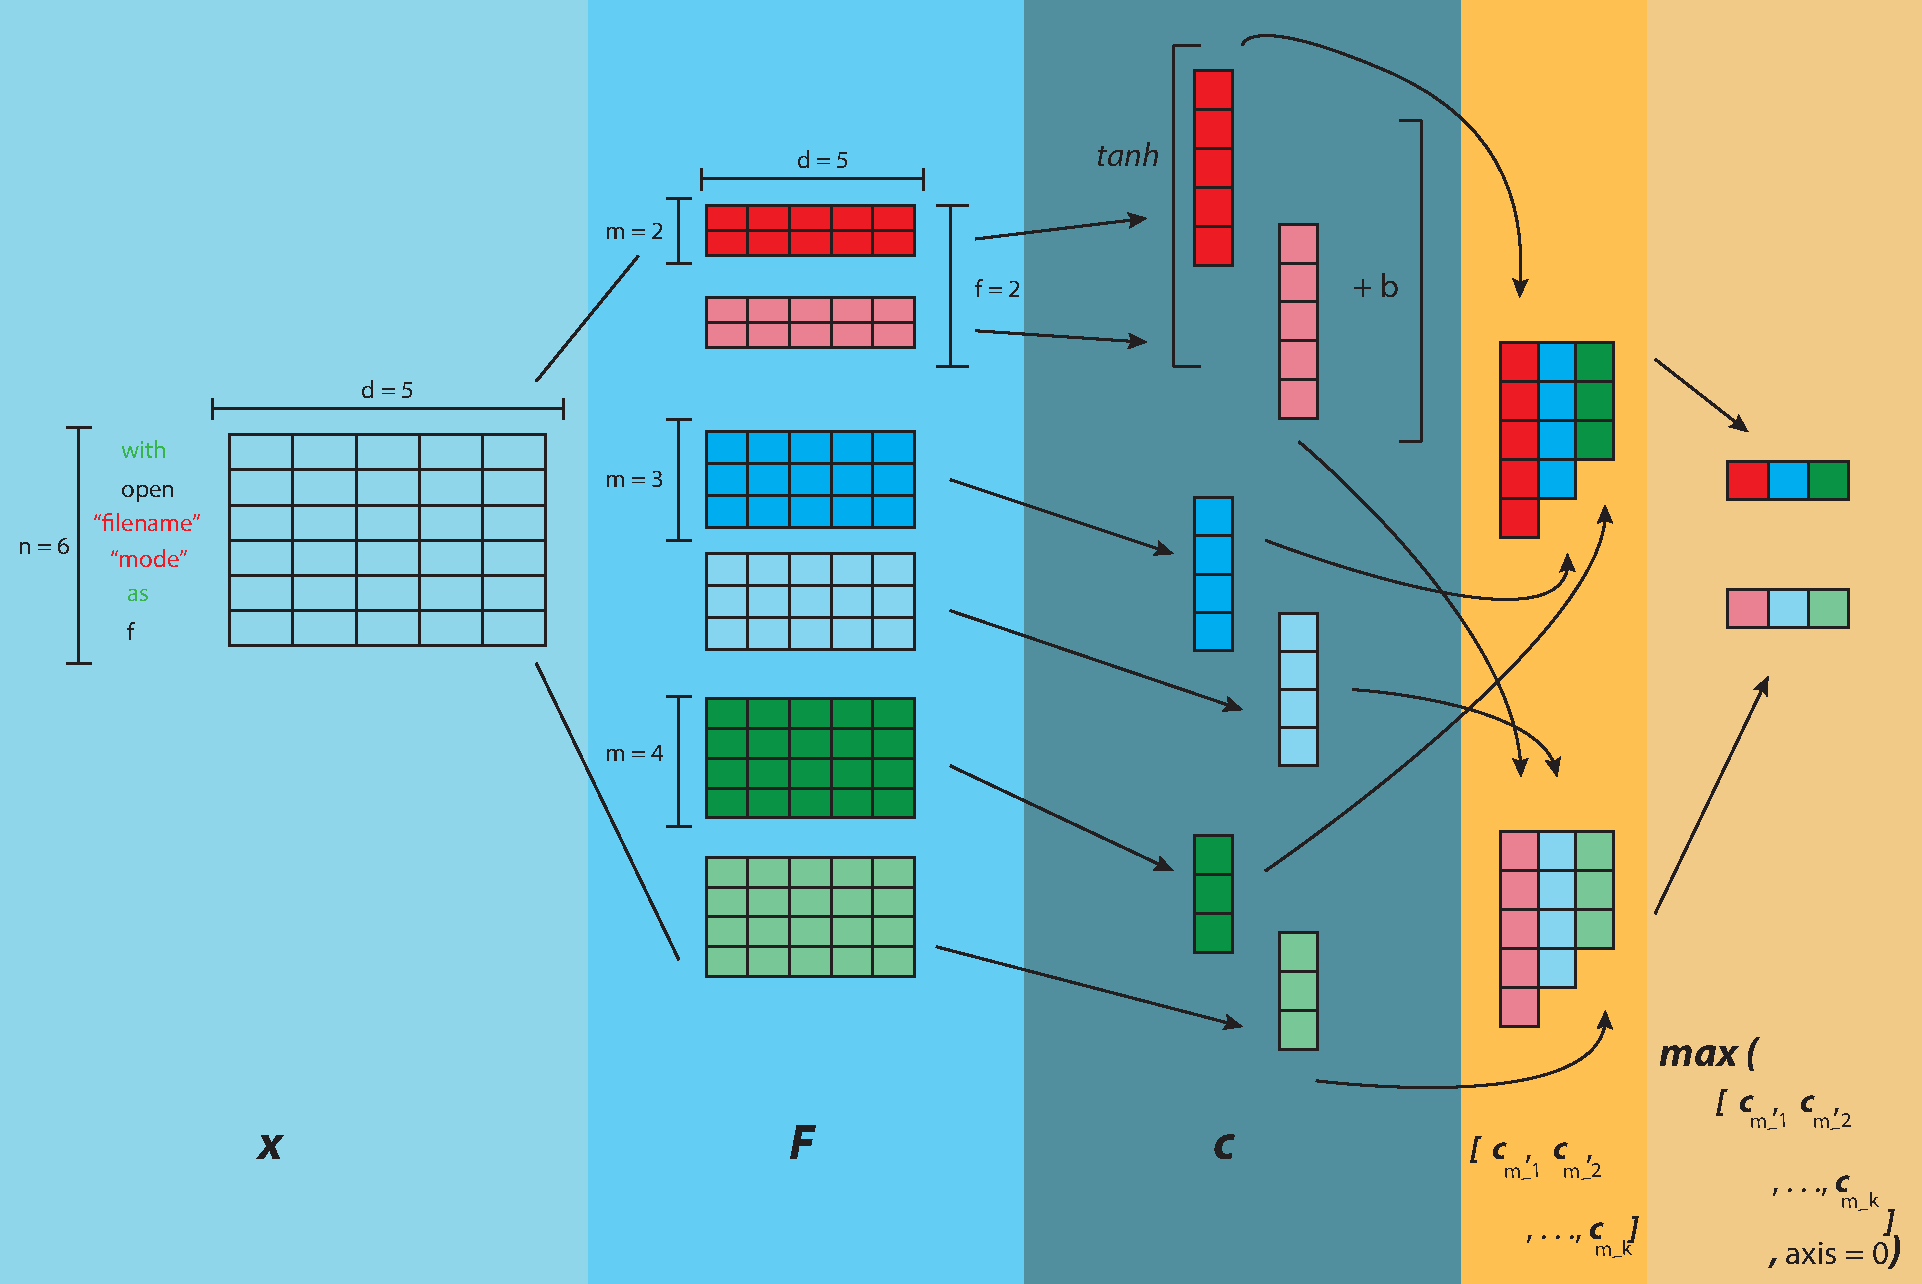
\includegraphics[width=1\textwidth]{figuras/cap-problema/cnn-architecture.pdf}
    \caption{Ilustração das 3 operações realizadas pela nossa arquitetura CNN para obter o vetor de representação final $\bm{c'}_{\bm{m}}$. Neste exemplo, utilizamos 3 filtros $\bm{F} \in \mathbb{R}^{m X d X f}$ com diferentes janelas $m$, onde $m = \{2, 3, 4\}$. Cada filtro tem tamanho $f = 2$. Temos um total de 6 filtros ao final. Cada filtro é aplicado a sentença $\bm{x} \in \mathbb{R}^{n X d}$, onde $n = 6$ e $d = 5$. O primeiro passo é a obtenção do vetor $\bm{c}$ de características. Posteriormente, é realização a operação de concatenação, no qual é obtido o vetor $\bm{c}_{\bm{m}}$, conforme descrito na operação~\ref{eq:concatenacao-cnn-cm}. Ao final, a operação \textit{max} é aplicada no eixo $0$, obtendo o vetor de representação final $\bm{c'}_{m}$. Este vetor $\bm{c'}_{m}$ será o nosso vetor de representação das nossas sentenças, i.e., o vetor de representação das questões e trechos de código-fonte. Figura adaptada do artigo de \cite{zhang-guide-convolutional-cnn-embedding-ilustration:2015}}
    \label{fig:cnn-architecture-proposal}
\end{figure}




\section{Função objetivo}
\label{sec:funcao-objetivo}

O nosso objetivo é encontrar um modelo que correlacione as questões as respostas em um mesmo espaço vetorial. Lembrando que as questões e os trechos de código serão representados por um vetor calculado a partir da nossa arquitetura CNN. Para encontrar este modelo, adotaremos a mesma abordagem utilizada por \cite{feng-2015}, o método \textit{pairwise}. O método \textit{pairwise} consiste em treinar o modelo para classificar as respostas corretas com uma pontuação maior do que as incorretas. Formalmente, o modelo será treinado do seguinte modo:

Seja $\mathbb{Q}$ um conjunto de questões e $\mathbb{C}$ um conjunto dos trechos de código-fonte. $\mathbb{Q}$ e $\mathbb{C}$ compõem o conjunto de dados de treinamento. O dado de entrada fornecido para o nosso modelo será uma tripla $<\bm{q}, \bm{c^{+}}, \bm{c^{-}}>$, onde $\bm{c^{+}} \in \mathbb{C}$ é uma resposta anotada como correta para a questão $\bm{q} \in \mathbb{Q}$ e $\bm{c^{-}} \in \mathbb{C}$ é uma resposta incorreta. O objetivo é induzir o nosso modelo a classificar $\bm{c^{+}}$ com uma pontuação maior que $\bm{c^{-}}$. Para isto, utilizaremos a seguinte função de custo \textit{hinge}:

\begin{equation}
J = max(0, m - h_{\theta}(\bm{q}, \bm{c^{+}}) + h_{\theta}(\bm{q}, \bm{c^{-}}))
\end{equation}

Onde $m$ é uma margem e $h_{\theta}$ é uma função de similaridade, e.g., \textit{cosine}. Lembrando que o objetivo em uma rede neural é minimizar a função custo $J$. Desta maneira, o modelo vai ser incentivado a satisfazer a seguinte condição: $h_{\theta}(\bm{q}, \bm{c^{+}}) - h_{\theta}(\bm{q}, \bm{c^{-}}) \geq m$. Quer dizer, a função \textit{hinge} induz o modelo a classificar as respostas corretas com uma pontuação maior do que as incorretas por uma certa margem $m$. 

Dado que estamos utilizando a função \textit{cosine} de similaridade, $h_{\theta}(\bm{q}, \bm{c})$ pode ser definido como $\{h_{\theta}(\bm{q}, \bm{c}) \in \mathbb{R} | -1 \leq h_{\theta}(\bm{q}, \bm{c}) \leq 1$\}, onde $\bm{q} \in \mathbb{Q}$, $\bm{c} \in \mathbb{C}$ e $-1$ indica vetores exatamente opostos e 1 vetores exatamente iguais. E conforme citado anteriormente, a nossa função $\mathbb{J}$ incentiva a seguinte condição: $h_{\theta}(\bm{q}, \bm{c^{+}}) \geq h_{\theta}(\bm{q}, \bm{c^{-}}) + m$. Desta forma, estamos estimulando os vetores $\bm{c^{+}}$ a ocuparem regiões próximas de $\bm{q}$, enquanto os vetores $\bm{c^{-}}$ serão estimulados a ocuparem regiões mais distantes. Este estímulo está de acordo com o nosso objetivo, que é encontrar um modelo que correlacione as questões as suas respostas.


\section{Considerações}

A nossa proposta apresentada neste capítulo foi a utilização de redes convolucionais na representação de questões e trechos de código-fonte. Conforme apresentado na Seção~\ref{sec:representacao-sentenca}, a nossa arquitetura utiliza as operações de convolução e \textit{maxpool}. Estas operações partem da hipótese de que função que deve ser aprendida contém apenas interações locais e são invariantes a pequenas translações. Para a tarefa de \textit{code retrieval}, a nossa hipótese, é que a identificação das interações locais entre as palavras pode auxiliar na obtenção de uma representação contextualizada. Por exemplo, para inferir o contexto do trecho de código a seguir, o CNN deveria ser capaz de identificar a interação entre as palavras \emph{csv} e \emph{writer} na linha 4, por exemplo. 

\begin{mypython-linenumber}{CNN}
import csv

with |\colorbox{green}{open}|("output.csv", "wb") as f:
    writer = |\colorbox{green}{csv}|.|\colorbox{green}{writer}|(f)
    writer.|\colorbox{green}{writerows}|(a)
\end{mypython-linenumber}

Um ponto observado por \cite{tom-young:trends-deep-learning-nlp} em outros trabalhos, é que o CNN, normalmente, não consegue inferir o contexto em sentenças curtas. Para o nosso conjunto de dados, isto é um problema, pois as questões são compostas em média por 9 palavras e no máximo 32. Já os trechos de código tem em média 50 palavras e no máximo 300. Uma forma de mitigar este problema é através do uso de um vetor de representação distribuída. No nosso caso, os vetores de entrada serão compostos por vetores de representação distribuída obtidos através do algoritmo não-supervisionado \textit{word2vec}.

Além disso, segundo \cite{Goodfellow-et-al-2016:convolutional-networks}, CNN não consegue fazer associações entre palavras muito distantes em uma sentença. No exemplo anterior, o CNN teria dificuldade para associar a declaração da biblioteca \emph{csv} na linha 1 com a função \emph{writerows} na linha 5. A nossa hipótese é que uma associação muito distante entre as palavras de uma sentença não seja tão importante para a recuperação de trecho de código-fonte no nosso conjunto de dados. O nosso conjunto de dados é formado por questões do tipo \textit{how-to-do-it} coletadas a partir do site \gls{sof}. Este tipo de questão normalmente contém respostas curtas e diretas  \citep{yao-2018}. Uma dependência distante entre as palavras seria apropriado, provavelmente, para questões e trechos de código que envolvam regras de negócio, por exemplo.


Ao optar por uma arquitetura, temos que levar em consideração as suas características inerentes e suas limitações. No caso do CNN, ele prioriza as interações locais ao invés de associações de palavras muito distantes. A nossa hipótese inicial é que esta característica seja mais importante para a recuperação de trecho de código-fonte no conjunto de dados que estamos utilizando. Dado estas características, reiteramos a nossa pergunta de pesquisa que pretendemos responder ao longo deste trabalho:

\begin{itemize}
    \item Será que o CNN é capaz de extrair as características latentes e mais importantes de modo a facilitar o modelo a encontrar uma correlação entre os trechos de código-fonte e as questões?
\end{itemize}

Indiretamente, dado que o CNN prioriza interações locais, estaremos respondendo as seguintes perguntas:
\begin{itemize}
    
        \item As interações locais auxiliam na aproximação das questões aos trechos de código-fonte?
        \item A partir das interações locais, é possível inferir o contexto do trecho de código?
\end{itemize}



O que entedemos por características latentes e importantes são palavras ou variáveis latentes que permitam inferir o contexto de um trecho de código. No exemplo anterior, as palavras \emph{csv}, \emph{writer} e \emph{writerows} permitem deduzir o contexto do trecho de código. Que no caso, refere-se a escrita dos valores de cada elemento de um vetor em um arquivo CSV. Nem sempre estas características são observáveis diretamente nos dados. Nestes casos, as redes deep learning capturam estas características através de variáveis latentes ou \textit{hidden}, $\bm{h}$. Através da variável \textit{hidden} $\bm{h}$, ela consegue identificar uma dependência indireta entre duas variáveis quaisquer $v_{i}$ e $v_{j}$ através da dependência direta entre $v_{i}$ e $\bm{h}$ e $\bm{h}$ e $v_{j}$ \citep{Goodfellow-et-al-2016:structured-probabilistic-models-for-deep-learning}.

Para avaliar se o modelo está inferindo o contexto do trecho de código corretamente, verificaremos se o modelo está aproximando as questões aos trechos de código que são respostas. Conforme descrito na Seção~\ref{sec:funcao-objetivo}, o modelo será induzido a fazer esta aproximação durante o treinamento através da função \textit{hinge}. Mas para saber se o modelo aprendeu, avaliaremos esta aproximação em outro conjunto de dados. No nosso caso, avaliaremos em um conjunto de dados anotados manualmente. O desempenho do modelo será medido através da métrica \acrshort{mrr} descrita no Capítulo~\ref{cap:experimento}. Um valor alto do MRR indica que o modelo está aproximando corretamente as questões aos trechos de código-fonte anotados como respostas. Para nós, isto é um indicativo de que o modelo está inferindo o contexto do trecho de código corretamente.
